\documentclass[12pt,twoside]{article}   
\usepackage{../light}

%  The solutions still need some work!

%\hidesolutions
\showsolutions

\begin{document}

\problemset{7}{October 19, 2006}{\textit{Monday October 23 at 8 PM}}

%%%%%%%%%%%%%%%%%%%%%%%%%%%%%%%%%%%%%%%%%%%%%%%%%%%%%%%%%%%%%%%%%%%%%%%%%%%%%%%

\begin{problem} 
You are thinking about retiring in the future, and are thinking about ways to
invest your money now. 

\bparts
\ppart
You decide to take advantage of a new tax deferred annuity (TDA).
You decide to contribute $m$ dollars at the beginning of each year for $n$ years to
the TDA. The interest rate for the TDA is $p$, the tax rate is $t$, but the nice thing is
that the interest you make through the TDA is tax-free. At the end of $n$ years you
withdraw your money, and then pay taxes at the same rate $t$, but only on the interest you've earned over the years. How much money do you have
at the end of $n$ years?

\solution{Due to interest, at the end of the first year, 
you have accumulated $m(1+p)$ dollars. 
At the end of the second year, 
you have accumulated $m(1+p)^2 + m(1+p)$ dollars, 
since both the previous amount and the new $m$ dollars you invest get interest.
Similarly, at the end of $n$ years you have $\sum_{i=1}^n m(1+p)^i$. 
Note that, since you have not yet taken the money out, you have not been taxed. Then, you withdraw the money, and are left with $\sum_{i=1}^n m(1+p)^i - t(\sum_{i=1}^n m(1+p)^i-nm) = (1-t)\sum_{i=1}^n m(1+p)^i + tmn$. The first part is just a geometric series, and evaluating it yields:
\begin{eqnarray*}
(1-t) \sum_{i=1}^n m(1+p)^i & = & m(1-t)\sum_{i=1}^n (1+p)^i\\
& = & (1-t)m \cdot (\frac{(1+p)^{n+1}-1}{(1+p)-1} - 1)\\
& = & (1-t)m \cdot (\frac{(1+p)^{n+1}-1}{p} -1).
\end{eqnarray*}
Thus, the total is $(1-t)m\cdot \frac{(1+p)^{n+1}-1}{p} + tmn$.
}

\ppart
Suppose you were instead to invest the $m$ dollars each year in a 
taxable fund with interest rate $p$ and annual tax rate $t$. 
In this case, at the end of each year, you are taxed on the interest
that you made that year.
How much money would you have after $n$ years?

\solution{At the end of the first year, you have $m(1+p)-tpm$ since you lose $tpm$ due to taxes at the end of the first year. 
At the end of two years you have 
$m(1+p-tp) + m(1+p-tp)(1+p) - tpm(1+p-tp) = m(1+p-tp) + m(1+p-tp)^2$. 
In general, at the end of $n$ years you have $\sum_{i=1}^n m(1+p-tp)^i$. This sum is a geometric series, and evaluating it yields:
\begin{eqnarray*}
\sum_{i=1}^n m(1+p-tp)^i & = & m \sum_{i=1}^n (1+p-tp)^i\\
& = & m \cdot (\frac{(1+p-tp)^{n+1}-1}{p-tp} - 1).
\end{eqnarray*}
}
\ppart
Suppose $n = 20$, $m= 10,000$, $t = .4$, and $p=.06$. How much more money do you make by using a TDA?

\solution{With a TDA, you make $313956$ dollars. On the other hand, with the second option you make $296009$ dollars. Thus, you make $17950$ more dollars.}
\eparts
\end{problem}

%%%%%%%%%%%%%%%%%%%%%%%%%%%%%%%%%%%%%%%%%%%%%%%%%%%%%%%%%%%%%%%%%%%%%%%%%%%%%%%

\begin{problem}
Find closed-form expressions for the following.  Show your work.

\bparts

\ppart{10}

\[
\sum_{i=0}^n \frac{9^i - 7^i}{11^i}
\]

\solution{Split the expression into two geometric series and then
apply the formula for the sum of a geometric series.
%
\begin{align*}
\sum_{i=0}^n \frac{9^i - 7^i}{11^i}
    & = \sum_{i=0}^n \left(\frac{9}{11}\right)^i -
        \sum_{i=0}^n \left(\frac{7}{11}\right)^i \\
    & = \frac{1 - \left(\frac{9}{11}\right)^{n+1}}{1 - \frac{9}{11}}
          - \frac{1 - \left(\frac{7}{11}\right)^{n+1}}{1 - \frac{7}{11}} \\
    & = - \frac{11}{2} \cdot \left(\frac{9}{11}\right)^{n+1}
        + \frac{11}{4} \cdot \left(\frac{7}{11}\right)^{n+1}
        + \frac{11}{4}
\end{align*}
}

\ppart{10}

\[
\sum_{i=0}^n \sum_{j=0}^m 3^{i+j}
\]

\solution{
\begin{align*}
\sum_{i=0}^n \sum_{j=0}^m 3^{i+j}
    & = \sum_{i=0}^n \left(3^i \cdot \sum_{j=0}^m 3^j\right) \\
    & = \left(\sum_{j=0}^m 3^j\right) \cdot \left(\sum_{i=0}^n 3^i\right)\\
    & = \left(\frac{3^{m+1} - 1}{2}\right) \cdot \left(\frac{3^{n+1} - 1}{2}\right)
\end{align*}
}

\ppart{10}

\[
\sum_{i=1}^n \sum_{j=1}^n (i + j)
\]

\solution{
\begin{align*}
\sum_{i=1}^n \sum_{j=1}^n (i + j)
    & = \left (\sum_{i=1}^n \sum_{j=1}^n i \right ) + \left (\sum_{i=1}^n \sum_{j=1}^n j \right )\\
    & = \left (\sum_{i=1}^n ni \right ) + \left (\sum_{i=1}^n  \frac{n(n+1)}{2} \right )\\
    & = \frac{2n^2(n+1)}{2}\\
    & = n^2(n+1)
\end{align*}
}

\ppart{10}
\[
\prod_{i=1}^n \prod_{j=1}^n 2^i \cdot 3^j
\]

\solution{
\begin{align*}
\prod_{i=1}^n \prod_{j=1}^n 2^i \cdot 3^j
    & = \left (\prod_{i=1}^n 2^{ni} \right ) \left (\prod_{j=1}^n 3^{nj} \right )\\
    & = 2^{n\sum_{i=1}^n i}3^{n\sum_{j=1}^n j}\\
    & = 2^{n^2(n+1)/2}3^{n^2(n+1)/2}
\end{align*}
}

\ppart{10}
In addition to expressing the following in closed form, compute the $\sim$ value for it.
\[
\prod_{i=1}^n (2i-1)
\]

\solution{
\begin{align*}
\prod_{i=1}^n (2i-1) 
    & = \frac{(2n)!}{\prod_{i=1}^n (2i)}\\
    & = \frac{(2n)!}{2^n \prod_{i=1}^n i}\\
    & = \frac{(2n)!}{2^n n!}
\end{align*}
Using Stirling's formula, $(2n)! \sim \sqrt{4\pi n} \left (\frac{2n}{e} \right )^{2n}$ and $n! \sim \sqrt{2 \pi n} \left (\frac{n}{e} \right )^n$. Thus the $\sim$ value of this expression is $\sqrt{2} \left (\frac{2}{e} \right )^n n^n$.
}
\eparts
\end{problem}

%%%%%%%%%%%%%%%%%%%%%%%%%%%%%%%%%%%%%%%%%%%%%%%%%%%%%%%%%%%%%%%%%%%%%%%%%%%%%%%

\begin{problem}
Pharaoh Aha I decides to build a ``pyramid'' in his honor consisting
of a single block:

\begin{center}
\includegraphics[height=0.5in]{aha1}
\end{center}

\noindent His successor, Aha II, trumps him by building a larger
pyramid:

\begin{center}
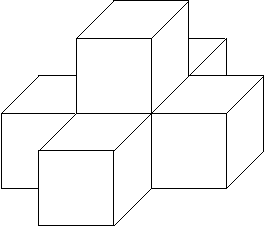
\includegraphics[height=1in]{aha2}
\end{center}

\noindent Not to be outdone, Aha III, builds a still-larger pyramid:

\begin{center}
\includegraphics[height=1.5in]{aha3}
\end{center}

\noindent If this continues, how many blocks will Pharoah Aha $n$
require?  Show your work.
\end{problem}

\solution{Vertical cuts divide the $n$th pyramid into $2n+1$
triangular slabs:

The number of blocks in a triangular slab of height $t$ is:
\begin{align*}
1 + 2 + \ldots + t + \ldots + 2 + 1
    & = t + 2 \sum_{i = 1}^{t-1} i \\
    & = t + 2 \cdot \frac{(t-1)t}{2} \\
    & = t^2
\end{align*}
Thus, the number of blocks in the $n$th pyramid is:
\begin{align*}
1^2 + 2^2 + \ldots + n^2 + \ldots + 2^2 + 1^2
    & = n^2 + 2 \sum_{i = 1}^{n-1} i^2 \\
    & = n^2 + 2 \cdot \frac{(n-1)n(2n-1)}{6} \\
    & = \frac{2n^3 + n}{3}
\end{align*}
}

%%%%%%%%%%%%%%%%%%%%%%%%%%%%%%%%%%%%%%%%%%%%%%%%%%%%%%%%%%%%%%%%%%%%%%%%%%%%%%%

\begin{problem}
Use integration bounds to compute the $\sim$ value of each of the following expressions. Prove your answer is correct.
\bparts
\ppart
$$\sum_{i=1}^n i^3$$
\solution{
\[
\int_0^{n} x^3 \ dx 
\quad \leq \quad
\sum_{i=1}^n i^3
\quad \leq \quad
\int_0^{n} (x+1)^3 \ dx
\]
Evaluating the integrals gives:
\[
\left. \frac{1}{4} x^4 \right|_0^n
\quad \leq \quad
\sum_{i=1}^{n} i^3
\quad \leq \quad
\left. \frac{1}{4} (x+1)^4 \right|_0^n
\]

\[
\frac{n^4}{4}
\quad \leq \quad
\sum_{i=1}^n i^3
\quad \leq \quad
\frac{(n+1)^4}{4}
\]

The left-hand side is $\sim \frac{n^4}{4}$, and the right-hand side is $\sim \frac{n^4}{4}$, and so $\sum_{i=1}^n i^3$ is $\sim \frac{n^4}{4}$.
}

\ppart
$$\sum_{i=1}^n i^{-1/3}.$$
\solution{
In this case, we need to be careful since $i^{-1/3}$ is not defined at $0$. However, at $1$ its value is just $1$. Therefore,
\[
1 + \int_1^{n} (x+1)^{-1/3} \ dx 
\quad \leq \quad
\sum_{i=1}^n i^{-1/3}
\quad \leq \quad
1+ \int_1^{n} x^{-1/3} \ dx
\]
Evaluating the integrals gives:
\[
1 + \left. \frac{3}{2} (x+1)^{2/3} \right|_1^{n}
\quad \leq \quad
\sum_{i=1}^{n} i^{-1/3}
\quad \leq \quad
1+ \left. \frac{3}{2} x^{2/3} \right|_1^n
\]
The left-hand side is $1 + \frac{3}{2}(n+1)^{2/3} - \frac{3}{2} \cdot 2^{2/3}$ and the right-hand side is $1+\frac{3}{2}n^{2/3} - \frac{3}{2}$. Note that the left-hand side is even larger than $1+\frac{3}{2}n^{2/3} - \frac{3}{2}$. We conclude that $\sum_{i=1}^n i^{-1/3} \sim \frac{3}{2}n^{2/3}$.
}

\eparts

\end{problem}

%%%%%%%%%%%%%%%%%%%%%%%%%%%%%%%%%%%%%%%%%%%%%%%%%%%%%%%%%%%%%%%%%%%%%%%%%%%%%%%

\begin{problem}
There is a bug on the edge of a 1-meter rug.  The bug wants to cross
to the other side of the rug.  It crawls at 1 cm per second.  However,
at the end of each second, a malicious first-grader named Mildred
Anderson \textit{stretches} the rug by 1 meter.  Assume that her
action is instantaneous and the rug stretches uniformly.  Thus, here's
what happens in the first few seconds:

\begin{itemize}

\item The bug walks 1 cm in the first second, so 99 cm remain ahead.

\item Mildred stretches the rug by 1 meter, which doubles its length.
So now there are 2 cm behind the bug and 198 cm ahead.

\item The bug walks another 1 cm in the next second, leaving 3 cm
behind and 197 cm ahead.

\item Then Mildred strikes, stretching the rug from 2 meters to 3
meters.  So there are now $3 \cdot (3 / 2) = 4.5$ cm behind the bug
and $197 \cdot (3/2) = 295.5$ cm ahead.

\item The bug walks another 1 cm in the third second, and so on.

\end{itemize}

Your job is to determine this poor bug's fate.

\bparts

\item During second $i$, what \textit{fraction} of the rug does the
bug cross?

\solution{During second $i$, the length of the rug is $100i$ cm and
the bug crosses 1 cm.  Therefore, the fraction that the bug crosses is
$1 / 100i$.}

\item Over the first $n$ seconds, what fraction of the rug does the
bug cross altogether?  Express your answer in terms of the Harmonic

number $H_n$.

\solution{The bug crosses $1/100$ of the rug in the first second,
$1/200$ in the second, $1/300$ in the third, and so forth.  Thus, over
the first $n$ seconds, the fraction crossed by the bug is:
%
\[
\sum_{k=1}^{n} \frac{1}{100k} = H_n / 100
\]
%
(This formula is valid only until the bug reaches the far side of the
rug.)}

\item Approximately how many seconds does the bug need to cross the
entire rug?

\solution{The bug arrives at the far side when the fraction it has
crossed reaches 1.  This occurs when $n$, the number of seconds
elapsed, is sufficiently large that $H_n / 100 \geq 1$.  Now $H_n$ is
approximately $\ln n$, so the bug arrives about when:
%
\begin{align*}
\frac{\ln n}{100} & \geq 1 \\
\ln n & \geq 100 \\
n & \geq e^{100} \approx 10^{43} \text{ seconds}
\end{align*}
}

\eparts

\end{problem}

%%%%%%%%%%%%%%%%%%%%%%%%%%%%%%%%%%%%%%%%%%%%%%%%%%%%%%%%%%%%%%%%%%%%%%%%%%%%%%%

\begin{problem}
Determine which of these choices 
\[
\Theta(n), \quad
\Theta(n^2 \log n), \quad
\Theta(n^2), \quad
\Theta(1), \quad
\Theta(2^n), \quad
\Theta(2^{n \ln n}), \quad
\text{none of these}
\]
describes each function's asymptotic behavior.  Proofs are not
required, but briefly explain your answers.

\bparts
\ppart  
\[
n + \ln n + (\ln n)^2
\]

\solution{Both $n > \ln n$ and $n > (\ln n)^2$ hold for all
sufficiently large $n$.  Thus, for all sufficiently large $n$:
\[
n < n + \ln n + (\ln n)^2 < n + n + n
\]
So $n + \ln n + (\ln n)^2 = \Theta(n)$.
}

\ppart
\[
e^{\pi^2}
\]
\solution{$e^{\pi^2}$ is a constant, that is, it does not vary with $n$. Therefore, $e^{\pi^2} = \Theta(1)$.
}

\ppart 
\[
\frac{n^2 + 2n - 3}{n^2 - 7}
\]

\solution{
Observe that:
\[
\lim_{n \to \infty} \frac{n^2 + 2n - 3}{n^2 - 7} = 1
\]
This means, that for all sufficiently large $n$, the fraction lies, for
example, between, $0.99$ and $1.01$ and is therefore $\Theta(1)$.}

\ppart 
\[
\sum_{i = 0}^n 2^{2i+1}
\]

\solution{Geometric sums are dominated by their largest term, which is
$2^{2n+1} = 2 \cdot 4^n$.  This is $\Theta(4^n)$, which does not
appear in the list provided.}

\ppart 
\[
\ln (n^2!)
\]

\solution{
By Stirling's formula:
\[
n^2! \sim \sqrt{2 \pi n^2} \left(\frac{n^2}{e}\right)^{n^2}
\]
Taking logarithms gives:
%
\begin{align*}
\ln(n^2!)
    & \sim \ln(\sqrt{2 \pi n^2} \left(\frac{n^2}{e}\right)^{n^2}) \\
    & = \ln(\sqrt{2 \pi n^2}) + \ln\left(\frac{n^2}{e}\right)^{n^2}
\end{align*}
%
The first term is tiny compared to the second, which we can rewrite as:
%
\[
\ln\left(\frac{n^2}{e}\right)^{n^2}
     = n^2 \ln\left(\frac{n^2}{e}\right) = \Theta(n^2 \ln n)
\]
}

\ppart
\[
\sum_{k=1}^{n} k \left(1 - \frac{1}{2^k}\right)
\]

\solution{The expression in parentheses is always at least $1/2$ and
at most $1$.  Thus, we have the bounds:
%
\[
\frac{1}{2} \sum_{k=1}^{n} k
\leq
\sum_{k=1}^{n} k \left(1 - \frac{1}{2^k}\right)
\leq
\sum_{k=1}^{n} k
\]
%
Since the first expression and the last are both $\Theta(n^2)$, so is
the one in the middle.}

\eparts

\end{problem}

\begin{problem}
This problem continues the study of the asymptotics of factorials.
\bparts
\ppart

Either prove or disprove each of the following statements.
\begin{itemize}
\item $n! = O((n+1)!)$
\item $n! = \Omega((n+1)!)$
\item $n! = \Theta((n+1)!)$
\item $n! = \omega((n+1)!)$
\item $n! = o((n+1)!)$
\end{itemize}

\solution{Observe that $n! = (n+1)!/(n+1)$, and thus $n! = o((n+1)!)$. Thus, $n! = O((n+1)!)$ as well, but the remaining statements are false.}

\ppart
Show that $n! = \omega \left (\frac{n}{3} \right )^{n+e}$.

\solution{By Stirling's formula:
\[
n! \sim \sqrt{2 \pi n} \left(\frac{n}{e}\right)^{n}
\]

On the other hand, note that $\left (\frac{n}{3} \right )^{n+e} = \left (\frac{n}{3} \right )^e \left (\frac{n}{3} \right )^n$. Dividing $n!$ by this quantity,
$$\frac{3^e\sqrt{2\pi}}{n^{e-1/2}} \cdot \left (\frac{3}{e} \right )^n,$$
we see that since $3 > e$, this expression goes to $\infty$. Thus, $n! = \omega \left (\frac{n}{3} \right )^{n+e}$.
}
\eparts
\end{problem}
 

%% %%%%%%%%%%%%%%%%%%%%%%%%%%%%%%%%%%%%%%%%%%%%%%%%%%%%%%%%%%%%%%%%%%%%%%%%%%%%%%%

\end{document}                            
